\documentclass{beamer} %

%%%BASICS
\usepackage[utf8]{inputenc}
\usepackage{csquotes}
\usepackage{graphicx}
\graphicspath{ {./Images/} }

%%%START THEME SETTINGS
\usetheme{Dresden}
\usecolortheme{beaver}
\usefonttheme{professionalfonts}
\setbeamertemplate{itemize item}{\color{red}$\blacksquare$}
%%%END THEME SETTINGS

%%%START APA
\usepackage[british]{babel}
\usepackage[backend=biber,style=apa]{biblatex}
\DeclareLanguageMapping{british}{british-apa}
%% APA citing
%% \cite{t} - Uthor und Richter, 2010
%% \textcite{t} - Uthor und Riter (2010)
%% \parencite{t} - (Uthor & Riter, 2010)
%% \parencite[Chapt.~4]{t} - (Uthor & Riter, 2010, S. 15)
%%%END APA


\title[The Effectiveness of Sunscreen]{Investigating the Impact of Concentration on Non-Nano Zinc Oxide as a Viable Sun Protector: A Comparative Analysis with Commercial Sunscreens}
\institute[ICR]{The Institute for Computing in Research}
\author{Natalia Marquez and Abigail Wilson*}

\begin{document}

\begin{frame}
  \titlepage
\end{frame}

%------------------------------------------------------

\section{The Main Question}
\begin{frame}\centering
  \frametitle{The Main Question}
  Is it possible to create a sunscreen that is just as effective as store-bought sunscreen and can concentration affect this?
\end{frame}

\section{Background}
\begin{frame}
  \frametitle{Background}
  \begin{itemize}
    \item What is UV?
    \item How Does Sunscreen Protect Us?
    \item Why Are We Using Zinc Oxide?
  \end{itemize}
\end{frame}

\subsection{Ultraviolet (UV)}
\begin{frame}\centering
  \frametitle{UV}
  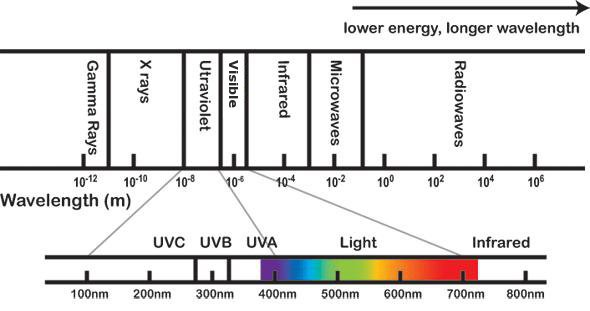
\includegraphics[scale = 0.7]{EMRSpectrum.jpg}
\end{frame}
\begin{frame}\centering
  \frametitle{UV and Cyclobutane Pyrimidine Dimers}
  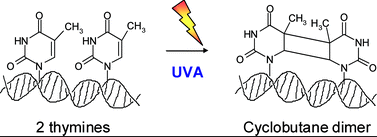
\includegraphics{CPD.png}
\end{frame}
\subsubsection{The UV Index}
\begin{frame}\centering
  \frametitle{The UV Index}
  
\includegraphics{UVIndex.png}
\end{frame}
\subsubsection{The UV Sensor}
\begin{frame}\centering
  \frametitle{The UV Sensor}
  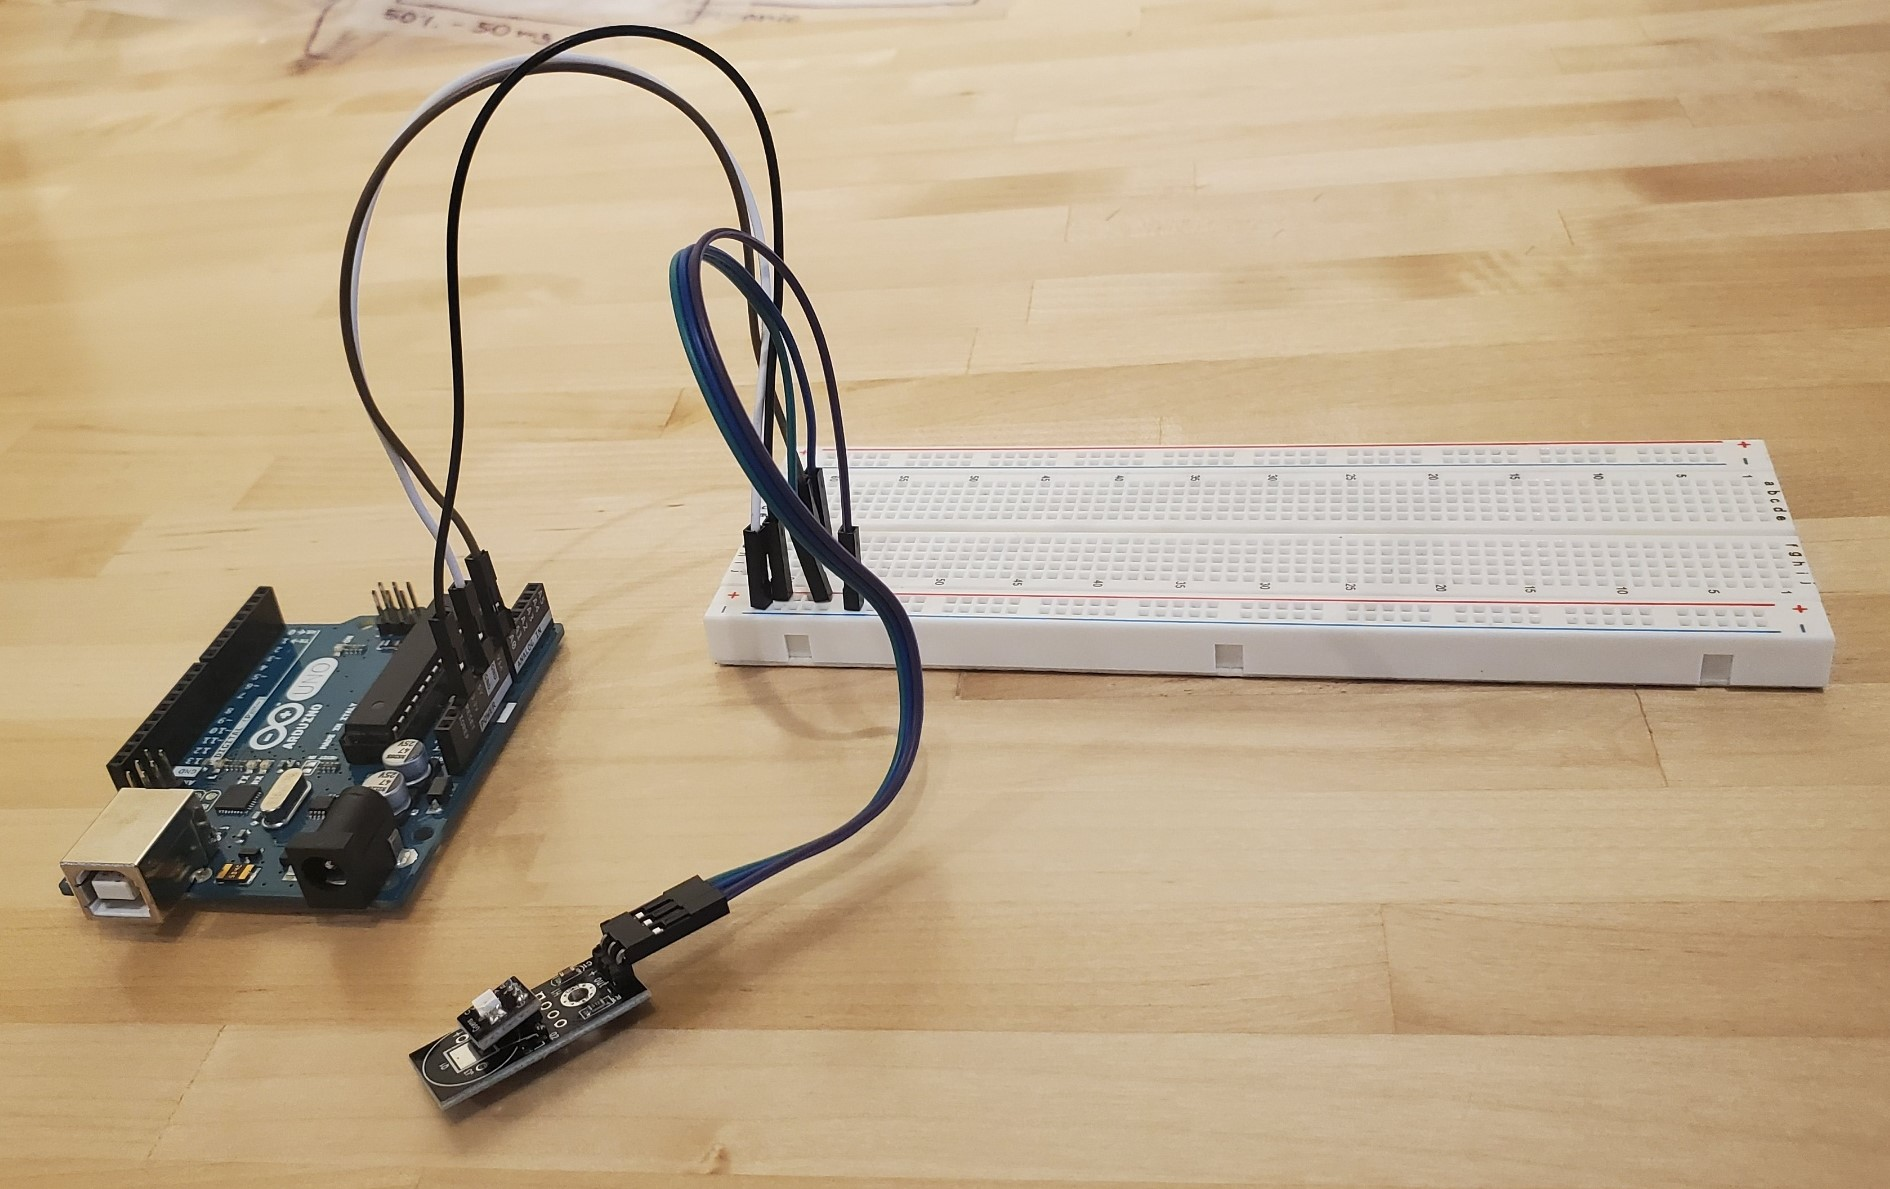
\includegraphics[scale = 0.2]{UVSensor.jpg}
\end{frame}

\subsection{Why Sunscreen Works}
\begin{frame}\centering
  \frametitle{Why Sunscreen Works}
  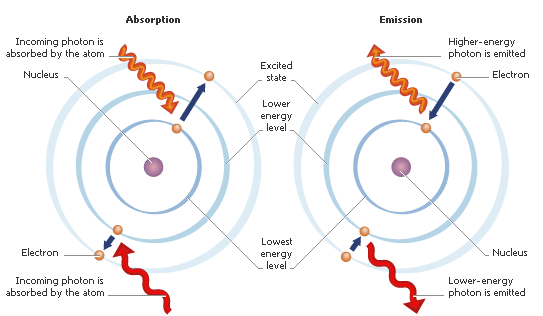
\includegraphics[scale = 0.5]{Absorption.png}
\end{frame}
\subsubsection{Possible Sunscreen Dangers}
\begin{frame}\centering
  \frametitle{Possible Sunscreen Dangers}
  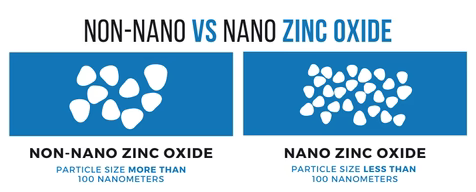
\includegraphics[scale = 0.65]{NonNanovsNanoZO.png}
\end{frame}
\subsubsection{The Sun Protection Factor}
\begin{frame}\centering
  \frametitle{The Sun Protection Factor}
  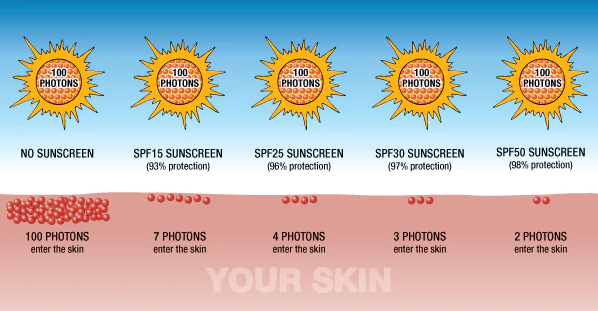
\includegraphics[scale = 0.5]{SPF.png}
\end{frame}
\subsubsection{Sun Protection and Concentration}
\begin{frame}\centering
  \frametitle{Sun Protection and Concentration}
  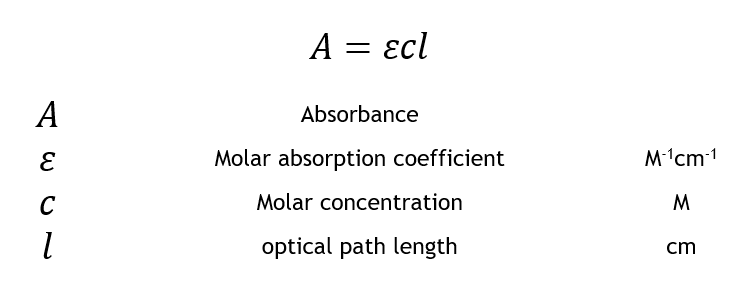
\includegraphics[scale = 0.65]{beerlambert.png}
\end{frame}
\subsection{Why Zinc Oxide?}
\begin{frame}\centering
  \frametitle{Why Zinc Oxide?}
  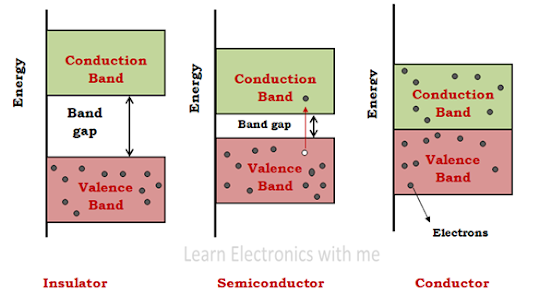
\includegraphics[scale = 0.5]{bandgap.png}
\end{frame}

\section{Materials and Methods}
\begin{frame}\centering
  \frametitle{Materials and Methods}
  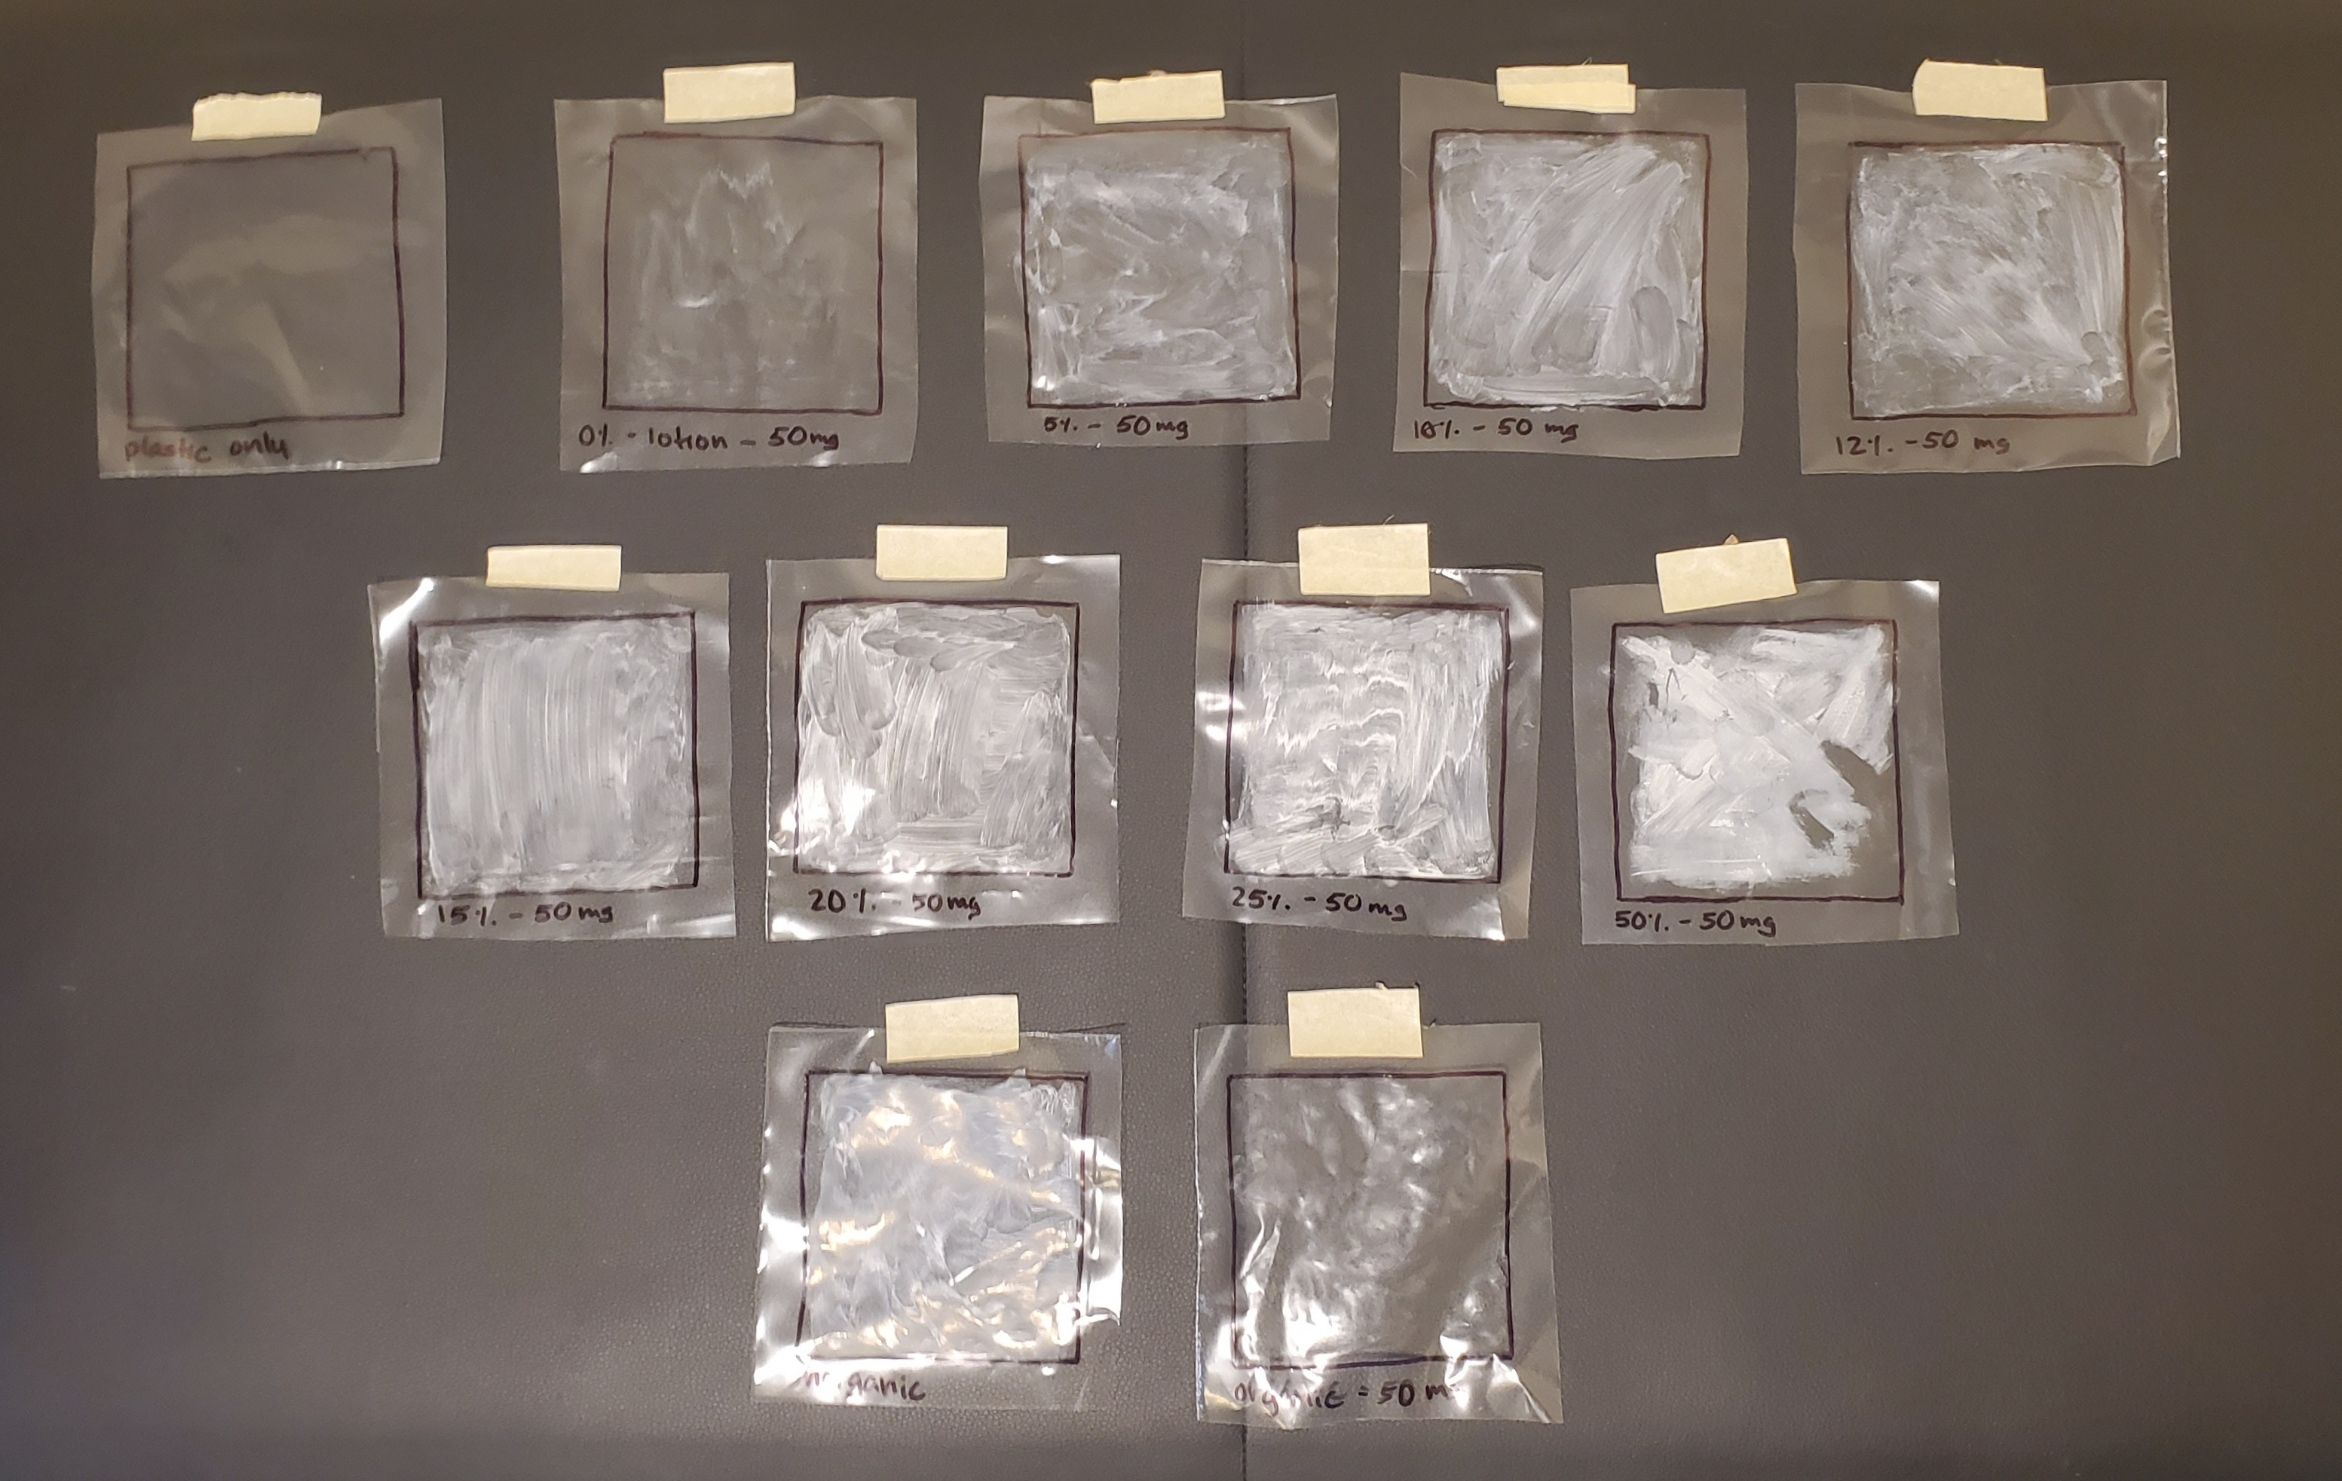
\includegraphics[scale = 0.1]{Sunscreens.jpg}
\end{frame}
\subsection{Experimental Design}
\begin{frame}\centering
  \frametitle{Experimental Design}
  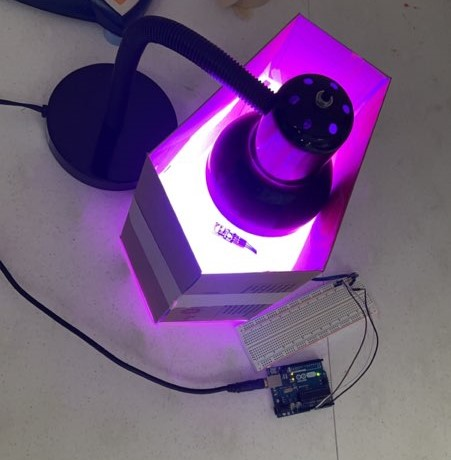
\includegraphics[scale = 0.5]{UVLamp.jpg}
\end{frame}

\section{Results and Discussion}
\begin{frame}\centering
  \frametitle{Results and Discussion}
  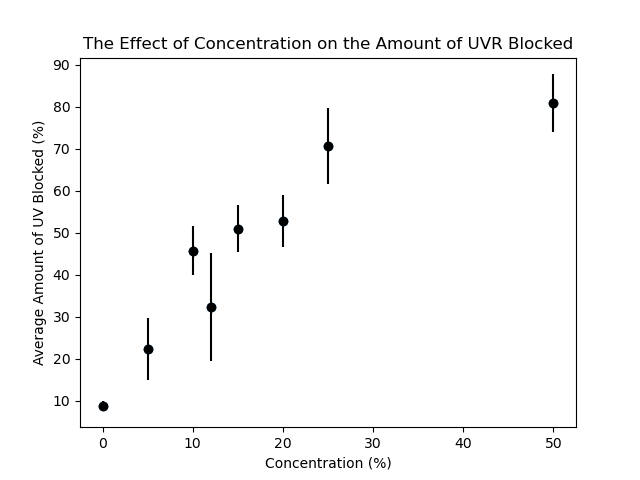
\includegraphics[scale = 0.5]{SunscreenDataPlotZO.png}
\end{frame}
\begin{frame}\centering
  \frametitle{Results and Discussion}
  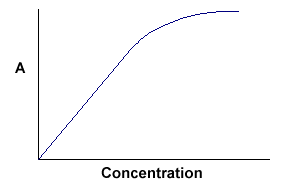
\includegraphics[scale = 0.75]{BLCurve.png}
\end{frame}
\begin{frame}\centering
  \frametitle{Results and Discussion}
  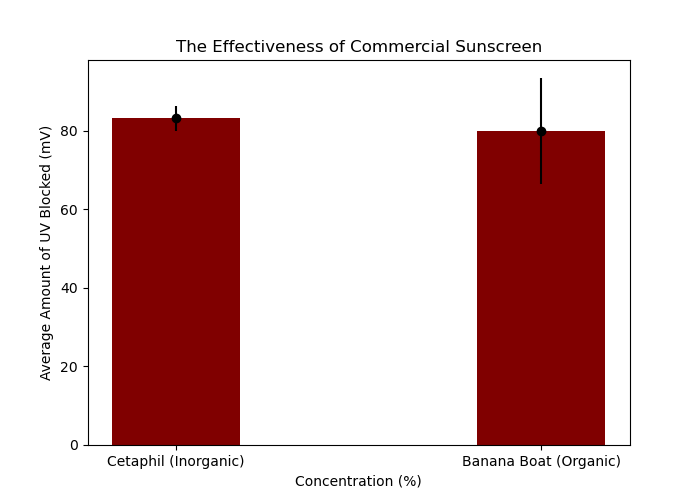
\includegraphics[scale = 0.5]{SunscreenDataPlotCommercial.png}
\end{frame}
\begin{frame}\centering
  \frametitle{Results and Discussion}
  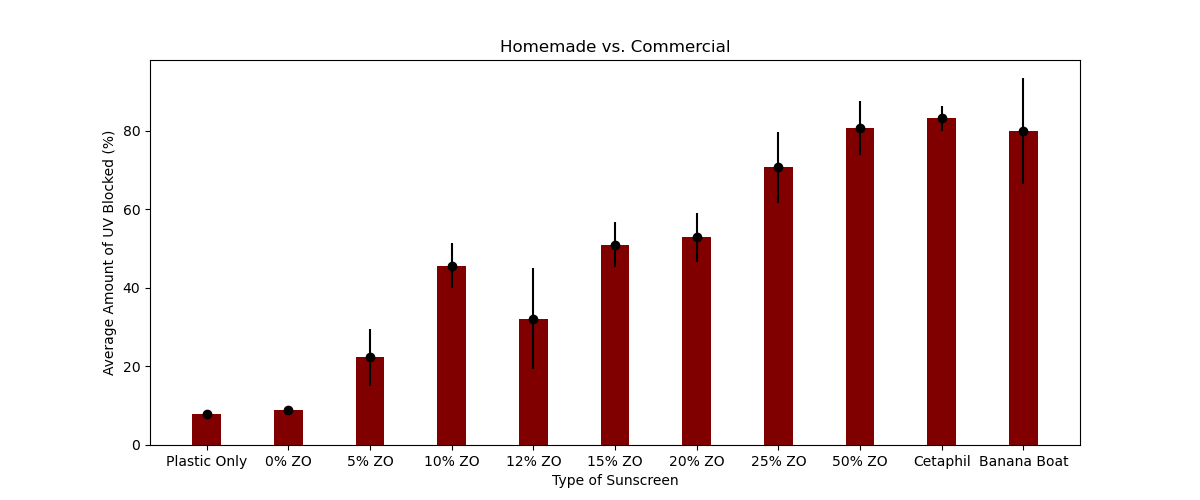
\includegraphics[scale = 0.4]{SunscreenDataPlot.png}
\end{frame}
\begin{frame}\centering
  \frametitle{Results and Discussion}
  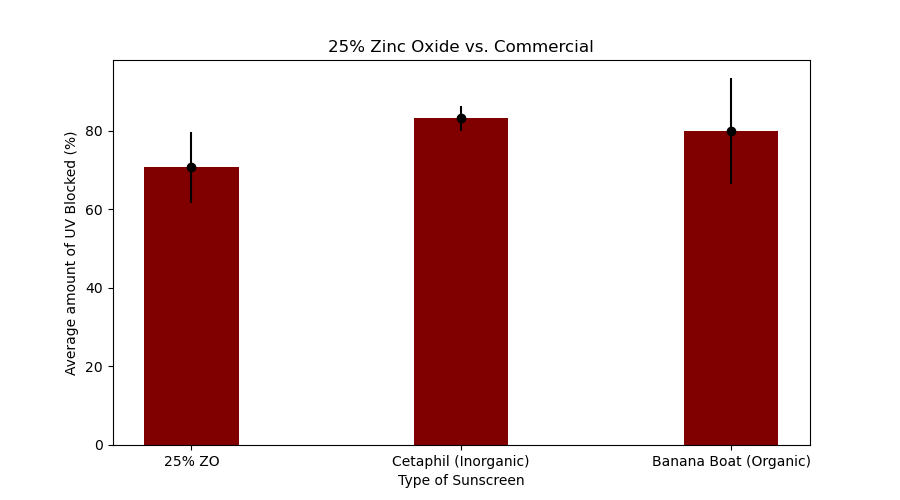
\includegraphics[scale = 0.5]{25ZOvsCommercialPlot.png}
\end{frame}

\section{Acknowledgements}
\begin{frame}\centering
  \frametitle{Acknowledgements}
  I would like to thank my mentor Abigail Wilson for her valued guidance, direction, and comfort. I would also like to thank Rhonda Crespo, Mark Galassi, and my fellow interns at the Institute for Computing in Research for their help and support. I would also like to thank Richard Pitman for writing my recommendation letter, as well as thanks to both Richard Pitman and Derek Buschman for helping to further my interest in the sciences and helping to teach me over these past 3 years.
\end{frame}
\begin{frame}\centering\Huge
  Thank you!
\end{frame}

\end{document}
